\documentclass[12pt]{article}

% set indentation
\usepackage{parskip}
%\setlength{\parindent}{16mm}

% for the figures
\usepackage{graphicx}
\usepackage{extsizes}
\usepackage{wrapfig}
% change margins
\usepackage{geometry}
\geometry{left=20mm,right=20mm,top=15mm,bottom=15mm}

% for the reference
\usepackage[sort]{natbib}
\usepackage{url}
\usepackage{placeins}
%\usepackage{authblk}
\usepackage{setspace}
\usepackage{tabularx}
%\doublespacing
% in preamble
%\usepackage{movie15}
% in documenet

\usepackage{authblk}
\usepackage{graphicx}
\usepackage{mathptmx} 
% My packages
\usepackage{parskip}
\usepackage{relsize, threeparttable}
\usepackage{array}
\usepackage{booktabs}
\usepackage{lscape}
\usepackage{tabularx}
\usepackage{makecell}
\usepackage{booktabs}
\usepackage{numprint}
\usepackage{amsmath}
\usepackage{mathtools}
\usepackage{amssymb}
\usepackage{multirow}
\setlength{\parindent}{16mm}
% for the figures
\usepackage{graphicx}
\usepackage{placeins}
% for the reference
\usepackage{natbib}
\usepackage{floatrow}
\usepackage{chngcntr}
\usepackage{url}
\usepackage{dutchcal}
%\usepackage{boondox-calo}
\usepackage{upgreek}
%\date{}
\usepackage{color,soul}
\usepackage{amsmath}

\setlength{\parindent}{0pt}
\definecolor{lightgrey}{rgb}{0.925, 0.925, 0.925}
\sethlcolor{lightgrey}







\title{Unravelling the contribution of financial and longevity risks to changes over time in life annuities}

\author[1]{Jes\'us-Adri\'an \'Alvarez\thanks{alvarez@sdu.dk}}

\author[2]{Andr\'es M. Villegas}

\affil[1]{{\small Interdisciplinary Centre on Population Dynamics, University of Southern Denmark} }

\affil[2]{\small{School of Risk and Actuarial Studies and ARC Centre of Excellence in Population Ageing Research (CEPAR)\\ UNSW Business School, Sydney, Australia}}
%\date{}

\begin{document}
\maketitle

{
\setcounter{tocdepth}{2}
%\tableofcontents
}



\begin{abstract}
	Actuaries and risk managers are interested in developing strategies to ensure that changes in interest rates do not affect the value of a portfolio (commonly known as immunization). Similarly, there is a long-standing tradition among demographers to measure how changes over time in mortality affect summary measures such as life expectancy. In this paper, we bring these two perspectives together. We develop a new decomposition method to quantify the contribution of changes in mortality and interest rates to the change in life annuity prices. We introduce neat and intuitive formulations that allow actuaries and risk managers to easily asses stochastic changes in financial and longevity risks embedded in their life annuities' portfolios. \\
	
	To illustrate our method, we look at the long-term development of life annuity prices using financial and mortality data from the United Kingdom since 1841. We found that there is clear interplay between longevity and financial risk, where the former one is at times masked by high financial risk. 
\end{abstract}
\newpage
\section{Introduction}\label{introduction}


Mortality and interest rates are the driving forces behind fluctuations over time in life annuity factors. Who contributes the most to such changes? mortality or interest rates? This question depends on many factors such as the onset age of calculation of life annuities, time frame of analysis and, of course, the population to be analysed. However, even by considering all those factors, there is not such a tool to disentangle the sources of stochastic change in life annuity factors. The main reason for this is that fluctuations in mortality and interest rates and their impact in life annuities have been widely studied separately but rarely together.[HERE WE SHOULD EMPHASISE WHY IS IT IMPORTANT TO HAVE A METHOD TO ASSESS TOGETHER THESE TWO ISSUES? BESIDES KNOWING WHAT CONTRIBUTES THE MOST, WHAT ELSE CAN WE GAIN BY USING THIS METHOD AND NOT USING OTHER MORE SOPHISTICATED ONES ADDRESSING ONLY LONGEVITY (E.G. LONGEVITY GREEKS)]

\subsection{Interest rate immunization}

Interest-rate immunization \citep{redington1951papers,fisher1971coping,shiu1990redington,santomero1997financial,courtois2007immunization} is the starting point for any study dealing with unexpected changes in interest rates (commonly known as financial risk). Duration (denoted by $D$), is the central quantity used in interest-rate immunization and it is defined as “the sensitivity of a life annuity (or any other financial product) to changes in the force of interest, $\delta$” \citep{milevsky2013life,charupat2016sluggish}. Modified and dollar durations are the most used types of durations in finance. Both assume parallel shifts in the force of interest (WE SHOULD ELABORATE MORE ON THIS TOPIC).




\subsection*{Demographic perspective on changes in mortality}

Does there exist a similar measure to duration that captures the sensitivity to changes in mortality rates?
Mathematical demographers and populations biologists \citep{leser1955variations,keyfitz1968introduction,keyfitz1977difference,demetrius1974demographic,mitra1978short,goldman1986new,Vaupel1986,hakkert1987life,fernandez2015entropy} have analysed this issue for many decades. In particular, \citet{leser1955variations,demetrius1974demographic,keyfitz1977difference} introduced an indicator known as the \textit{life table entropy} (denoted by $H$), that  “measures changes in life expectancy consequent on a proportional change in the force of mortality, $\mu$”. The higher the life table entropy; the higher the sensitivity of life expectancy to mortality rates \citep{vaupel2011life,aburto2019threshold,aburto2020dynamics}.


Several demographers have also been interested in understanding the sources of fluctuations over time in life expectancy \citep{arriaga1984measuring,pollard1988decomposition,beltran2008integrated,beltran2011unifying}. Key among these contributions is the work done by \citet{Vaupel2003} who develop a neat method in continuous time to separate changes in life expectancy over time in terms of the general pace of mortality improvement, $\bar{\rho}$, and the entropy, $H$. The advantage of \citet{Vaupel2003} decomposition method relies on the fact that it allows further decomposition of age-specific and cause-specific contributions into the average pace of mortality improvement and entropy.


\subsection*{Longevity risk immunization}



The concept of entropy \citep{leser1955variations,demetrius1974demographic,keyfitz1977difference} was first extended to the case of life annuity factors by \citet{Haberman2011}. They define the entropy as the “sensitivity of a life annuity to proportional changes in the force of mortality”. The entropy is particularly useful in the measurement of longevity risk (unexpected changes of mortality).


Indeed, there is an growing line of research dealing with longevity risk that has used the entropy\footnote{with the name of mortality durations but it is essentially the same formulation} in the context of mortality rate immunization\footnote{similar to interest-rate immunization, mortality-rate immunization is defined as a set of strategies to ensure that the value of a portfolio will be little affected in response to changes in mortality rates}. In particular, \citet{wang2010optimal,tsai2011actuarial,Tsai2013a,Li2011} derive discrete formulas for life annuity entropy and convexities assuming constant and proportional changes in the force of mortality, $\mu$. Mortality-rate immunization has been recently extended to different types of life insurance and annuity products \citep{li2012key,Li2012,Wong2015,Luciano2015,levantesi2018natural}. The growing interest on mortality-rate immunization is due to the current scenario that developed countries are facing: low interest rates and continuous mortality improvements. These two factors expose life annuities (and other life contingent products) to higher longevity risk, allowing the capital market of mortality-link securities to grow \citep{blake2019still}.






\subsection*{Bringing both perspectives together}

Literature on analysis of sensitivity in mortality (mostly developed by mathematical demographers) and literature on sensitivity to interest rates (mostly developed by actuaries and financial managers) have remained largely disconnected\footnote{with exception of \citet{Haberman2011} that made clear the links between both literatures}. Paradoxically, both strands of literature direct efforts at the same objective: gain a better understanding of the inherent sources of change in life contingent quantities. Recently, \citet{lin2020natural} made strides on this regard by deriving discrete formulas to calculate sensitivity of life annuities (and whole life insurances) to simultaneous changes mortality and interest rates. They introduced a synthetic variable called 'the force of mortality-interest`, which results from the addition of the force of mortality and interest ($\mu^*=\mu+\delta$). While the application of \citet{lin2020natural} is interesting since it combines sensitivity in mortality and interest rates, it is unlikely that $\mu$ and $\delta$ change at the same pace over time.

In this study, we bring together the demographic and actuarial perspectives to the analysis of changes in life annuities. We develop a new decomposition method to quantify the contribution of stochastic changes in mortality and interest rates to stochastic changes in life annuity prices. We introduce neat and intuitive formulations that allow actuaries and risk managers to easily asses stochastic changes in financial and longevity risks embedded in their life annuities' portfolios. To illustrate our method, we first look at the long-term development of life annuity prices using financial and mortality data from the United Kingdom since 1841. Next, we forecast trends in mortality and interest rates under various scenarios to gain insights about how both components interplay in future life annuity prices. From the actuarial perspective, our formulations are useful in devising strategies for better risk management (longevity and financial) by levering on well-known results from mathematical demography and immunization.






\section{Preliminaries}\label{preliminaries}

All of the quantities expressed here vary over time period $t$. According to standard actuarial notation, we define the following quantities:

\begin{itemize}

\item
\(\mu(x,t)\) is the force of mortality at age \(x\) in time $t$.

\item
$_sp_x(t)=e^{-\int_{0}^{s}\mu(x+y,t)dy}$ is the time $t$ period survival probability from age \(x\) to age \(x+s\). 


\item
\(\delta(s,t)\) is the time $t$ forward force of interest at maturity $s$. This measure is a general form to express the term-structure of interest rates.

\item 

${v}(s,t)=e^{-\int_{0}^{s}\delta(y,t)dy}$ is the time $t$ discount factor, for a cash-flow payable at maturity $s$.

\end{itemize}

The derivative with respect to time $t$ is denoted by adding a point on top of the function of interest. For example, time derivatives for the forces of mortality and interest are expressed as:

\begin{equation} \label{eq:mudot}
\dot{\mu}(x,t)\equiv\frac{\partial\mu(x,t)}{\partial t},
\end{equation}

and 

\begin{equation} \label{eq:mudot}
\dot{\delta}(s,t)\equiv\frac{\partial\delta(s,t)}{\partial t}.
\end{equation}



The rate of mortality improvement (or progress in reducing mortality) is defined as


\begin{equation} \label{eq:rho}
\rho(x,t)=-\frac{\frac{\mu(x,t)}{\partial t}}{\mu(x,t)} = - \frac{\dot{\mu}(x,t)}{\mu(x,t)}.
\end{equation}

Similarly, the relative change in interest rates over time is captured by 


\begin{equation} \label{eq:phi}
\upvarphi(s,t)=-\frac{\frac{\delta(s,t)}{\partial t}}{\delta(s,t)} = -\frac{\dot{\delta}(s,t)}{\delta(s,t)}.
\end{equation}


The actuarial present value of a continuous life annuity at age $x$ evaluated at time $t$ is given by

\begin{equation}\label{eq:Annuity}
\bar{a}_x(t) = \int_0^\infty {}_sp_x(t) {v}(s,t)ds = \int_0^\infty {}_sE_x(t) ds,
\end{equation}

where ${}_sE_x(t)={}_sp_x(t) {v}(s,t)$. 



A life annuity deferred $s$ years starting to be paid at age $x+s$ is expressed as


\begin{equation}\label{eq:DefAnnuity}
{}_s|\bar{a}_x(t) = {}_sE_x(t) \bar{a}_{x+s}(t).
\end{equation}


\section{Dynamics of a life annuity}


We are interested on measuring changes in $\bar{a}_x(t)$ with respect to the time variable $t$. To achieve this aim, we first need to describe how $\bar{a}_x(t)$ reacts to changes in the forces of mortality and interest. We denote the \textit{entropy of a life annuity}\footnote{\cite{Tsai2011,Tsai2013a,Lin2020} denoted this measure as \textit{mortality duration}. We reserve the term duration to denote changes in $\bar{a}_x(t)$ with respect to interest rates.} as the measure that captures changes in $\bar{a}_x(t)$ with respect to $\mu(x,t)$. Formally, it is defined as 

\begin{equation}\label{eq:EntropyGeneral}
{H}_{x}(t) = \frac{ \frac{\partial \bar{a}_x(t) }{\partial \mu(x,t)}}{\bar{a}_x(t)}.
\end{equation}

The measure that captures the sensitivity of $\bar{a}_x(t)$ to changes in interest rates is commonly known as \textit{duration} and it is the foundation of interest rates' immunization. For a life annuity, it is defined as the relative derivative of the annuity factor with respect to changes in the force of interest \citep{Milevsky2012,Milevsky2012a}:


\begin{equation}\label{eq:DurationGeneral}
{D}_{x}(t) = \frac{ \frac{\partial \bar{a}_x(t) }{\partial \delta(s,t)}}{\bar{a}_x(t)}.
\end{equation}

Greater values for ${H}_{x}(t)$ and ${D}_{x}(t)$ indicate that $\bar{a}_x(t)$ is highly sensitive to changes in $\mu(x,t)$ and $\delta(s,t)$ respectively. The entropy and the duration of a life annuity can be measured either by assuming constant or proportional changes in $\mu(x,t)$ and $\delta(s,t)$. In the following section we develop formulations for both cases. 



\subsection{Changes in $\bar{a}_x(t)$ with respect to $\mu(x,t)$}

The entropy of a life annuity is denoted by ${H}^{c}_{x}(t)$ when changes in $\mu(x,t)$ are held constant at all ages and by ${H}^{p}_{x}(t)$ when  changes are performed proportional. Based on the results developed by \citet{Tsai2013a} and \citet{Lin2020}, when $\mu(x,t)$ is changed constantly to $\mu(x,t)+\gamma$ such that $\gamma$ is a small number (see proof in the Appendix), the entropy of $\bar{a}_x(t)$ becomes

\begin{equation}\label{eq:EntropyC}
{H}^{c}_{x}(t) = -\frac{\int_{0}^\infty s {}_sp_x(t) {v}(s,t) ds}{\bar{a}_x(t)}=\frac{{h}^{c}_{x}(t)}{\bar{a}_x(t)},
\end{equation}

where ${h}^{c}_{x}(t)=-\int_{0}^\infty s {}_sp_x(t) {v}(s,t) ds$. The term ${h}^{c}_{x}(t)$ is expressed in absolute (monetary) terms, whereas the entropy ${H}^{c}_{x}(t)$ is dimensionless because it does not depend on the absolute value of $\bar{a}_x(t)$.


In two separate articles, \citet{Haberman2011} and \citet{Tsai2013a} show that when changes in $\mu(x,t)$ are assumed to be proportional to a small number $\gamma$ such that $\mu(x,t)(1+\gamma)$, the entropy of $\bar{a}_x(t)$ becomes

\begin{equation} \label{eq:EntropyP}
{H}^{p}_{x}(t) = -\frac{ \int_{0}^{\infty}{}_sp_x(t)\ln[{}_sp_x(t)] {v}(s,t) ds}{\int_0^\infty {}_sp_x(t) {v}(s,t) ds}.
\end{equation}


Alternatively, we show (see proof in Section \ref{sec:EntropyAlt} of the Appendix) that Equation \ref{eq:EntropyP} can be expressed as

\begin{equation} \label{eq:EntropyP2}
\begin{split}
{H}^{p}_{x}(t) &=  \frac{\int_0^\infty \mu(x+s,t)   {}_s|\bar{a}_x(t) ds}{\bar{a}_x(t)} =  \frac{{h}^{p}_{x}(t)}{\bar{a}_x(t)}, 
\end{split}
\end{equation}

where ${h}^{p}_{x}(t)=\int_0^\infty \mu(x+s,t)   {}_s|\bar{a}_x(t) ds$. Analogous to the case where changes are assumed to be constant, quantities ${h}^{p}_{x}(t)$ and ${H}^{p}_{x}(t)$ are expressed in absolute and relative terms respectively. The formulations shown in this section are closely related to the ones developed in the mortality immunization literature \citep{Tsai2013a,Lin2020}. We extended them to the continuous case.

 
 

\subsection{Changes in $\bar{a}_x(t)$ with respect to $\delta(s,t)$}

 Similar to the entropy, changes in $\bar{a}_x(t)$ with respect to $\delta(s,t)$ can be assumed to be either constant or proportional. Duration assuming constant changes in $\delta(s,t)$ is denoted by ${D}^{c}_{x}(t)$, whereas ${D}^{p}_{x}(t)$ refers to the duration assuming proportional changes. For the former case we have that:



\begin{equation}\label{eq:DurationC}
\begin{split}
{D}^{c}_x(t)&= -\frac{\int_0^\infty s {}_sp_x(t) {v}(s,t)ds}{\bar{a}_x(t)} \\
&= \frac{{d}^{c}_x(t)}{\bar{a}_x(t)},
\end{split}
\end{equation}

where ${d}^{c}_x(t)=-\int_0^\infty s {}_sp_x(t) {v}(s,t)ds$. Thus, assuming constant changes in $\delta(s,t)$ results into common types of duration known in finance as \textit{dollar duration}, ${d}^{c}_x(t)$, and \textit{modified duration}, ${D}^{c}_x(t)$ (see \citet{Milevsky2012} and \citet{Tsai2013a} for further details). It is worth noting that Equations \ref{eq:EntropyC} and \ref{eq:DurationC} are identical such that ${d}^{c}_x(t)={h}^{c}_{x}(t)$. This means that constant (parallel) changes in the force of mortality have essentially the same effect as parallel changes in the force of interest.


Assuming proportional changes in $\delta(s,t)$ (see proof in Section \ref{sec:DurProp} of the Appendix) results in: 


\begin{equation}\label{eq:DurationP}
\begin{split}
{D}^{p}_{x}(t) &= -\frac{\int_0^\infty {}_sp_x(t) v(s,t) \ln(v(s,t))ds}{\bar{a}_x(t)}. \\
\end{split}
\end{equation}


Note that when assuming constant force of mortality such that $v(s,t)=e^{-\delta(t)s}$, we have that ${D}^{p}_{x}(t)=\delta(t){D}^{c}_{x}(t)$,


\begin{equation}\label{eq:DurationCP}
\begin{split}
{D}^{p}_{x}(t) &= -\frac{\int_0^\infty {}_sp_x(t) v(s,t) \ln(v(s,t))ds}  {\bar{a}_x(t)} \\
&=- \delta(t)\frac{\int_0^\infty s{}_sp_x(t) e^{-\delta(t)s}  ds}{\bar{a}_x(t)} \\
& = \delta(t){D}^{c}_{x}(t).
\end{split}
\end{equation}

Equation \ref{eq:DurationP} can also be re-expressed as:

\begin{equation}\label{eq:DurationP2}
\begin{split}
{D}^{p}_{x}(t) &= \frac{\int_0^\infty \delta(s,t) {}_s|\bar{a}_x(t)ds} {\bar{a}_x(t)} \\
                 &= \frac{{d}^{p}_{x}(t)}{\bar{a}_x(t)}.
\end{split}
\end{equation}


where ${d}^{p}_{x}(t)=\int_0^\infty \delta(s,t) {}_s|\bar{a}_x(t) ds$. 




\section{Time derivative of $\bar{a}_x(t)$} \label{sec:timderiv}

We compute the derivative of $\bar{a}_x(t)$ with respect to the time variable $t$, $\dot{\bar{a}} _x(t)=\frac{\partial \bar{a}_x(t)}{\partial t}$, such that

\begin{equation}\label{eq:TimeDeriv}
\begin{split}
\dot{\bar{a}} _x(t) &= \int_0^\infty {}_s\dot{p}_x(t) v(s,t)ds +\int_0^\infty {}_sp_x(t) \dot{v}(s,t)ds.\\
\end{split}
\end{equation}


To develop a closed-form solution for Equation \ref{eq:TimeDeriv} we consider the general case where $_sp_x(t)=e^{-\int_{0}^{s}\mu(x+y,t)dy}$ and ${v}(s,t)=e^{-\int_{0}^{s}\delta(s,t)dy}$. We analyse separately each of the two terms in the right side of Equation \ref{eq:TimeDeriv}. Let us first focus on the first term:


\begin{equation}\label{eq:TimeDerivP1}
\begin{split}
\int_0^\infty {}_s\dot{p}_x(t) v(s,t) &= \int_0^\infty   v(s,t) e^{-\int_0^{s}\dot{\mu}(x+y,t)dy}ds\\
&= -\int_0^\infty   v(s,t) {}_sp_x(t)\int_0^{s}\dot{\mu}(x+y,t)dyds\\
&= -\int_0^\infty  \dot{\mu}(x+s,t) \int_s^{\infty} v(y,t) {}_yp_x(t) dyds\\
&= - \int_0^\infty \dot{\mu}(x+s,t)   {}_sE_x(t) \bar{a} _{x+s}(t) ds\\
&= \int_0^\infty \rho(x+s,t) \mu(x+s,t)   {}_s|\bar{a}_x(t) ds\\
\end{split}
\end{equation}


The second part equals:

\begin{equation}\label{eq:TimeDerivP2}
\begin{split}
\int_0^\infty {}_sp_x(t) \dot{v}(s,t)ds &= \int_0^\infty {}_sp_x(t)  e^{-\int_0^{s}\dot{\delta}(y,t)dy}ds\\
&= -\int_0^\infty {}_sp_x(t) v(s,t) \int_0^{s}\dot{\delta}(y,t)dy ds\\
&= -\int_0^\infty  \dot{\delta}(s,t)\int_s^{\infty} {}_yp_x(t) v(y,t) dy ds\\
&= \int_0^\infty  \upvarphi(s,t) \delta(s,t)  {}_s|\bar{a}_x(t) ds\\
\end{split}
\end{equation}


Thus, $\dot{\bar{a}} _x(t)$ can be expressed as


\begin{equation}\label{eq:TimeDerivP3}
\begin{split}
\dot{\bar{a}}_{x}(t) &=  \int_0^\infty \rho(x+s,t) \mu(x+s,t){}_s|\bar{a}_x(t) ds +\int_0^\infty  \upvarphi(s,t) \delta(s,t)  {}_s|\bar{a}_x(t) ds\\
&= \int_0^\infty \rho(x+s,t) {}_sM_x(t)  ds +\int_0^\infty  \upvarphi(s,t) {}_sW_x(t)  ds,
\end{split}
\end{equation}


where ${}_sM_x(t)= \mu(x+s,t){}_s|\bar{a}_x(t)$ and ${}_sW_x(t)=\delta(s,t)  {}_s|\bar{a}_x(t)$. We can express Equation \ref{eq:TimeDerivP3} in terms of the duration and entropy


\begin{equation}\label{eq:TimeDerivP}
\begin{split}
 \acute{\bar{a}}_x(t) = \frac{\dot{\bar{a}}_x(t)}{\bar{a}_x(t)}  = 
 \underbrace{\bar{\rho}_x(t){H}^{p}_x(t)}_\text{longevity component}
 +\underbrace{\bar{\upvarphi}(t){D}^{p}_x(t),}_\text{financial component}
\end{split}
\end{equation}

where $\bar{\rho}_x(t)= \frac{\int_0^\infty \rho(x+s,t) {}_sM_x(t)  ds}{\int_0^\infty  {}_sM_x(t)ds}$ and 
$\bar{\upvarphi}(t)= \frac{\int_0^\infty \upvarphi(s,t) {}_sW_x(t)  ds}{\int_0^\infty {}_sW_x(t) ds}$ are the weighted average paces of change in mortality and interest rates respectively. Functions $\bar{\rho}_x(t)$ and $\bar{\upvarphi}(t)$ capture the stochastic change in the forces of mortality and interest whereas ${H}^{p}_x(t)$ and ${D}^{p}_x(t)$ capture the sensitivity due to changes in $\mu$ and $\delta$. In other words, Equation \ref{eq:TimeDerivP} entails that changes over time in $\bar{a}_x(t)$ are driven by $\bar{\rho}_x(t)$ and $\bar{\upvarphi}(t)$, which are modulated by ${H}^{p}_x(t)$ and ${D}^{p}_x(t)$ respectively. Equation \ref{eq:TimeDerivP} is an extension of the decomposition formula to changes over time in life expectancy developed by \citet{Vaupel2003}. Here we extended it to life annuities.


\subsection{Age and term decomposition}

Equation \ref{eq:TimeDerivP} gives a way of understanding the sensitivity of the value of an annuity to overall changes in mortality and in the the term structure of interest rates. However, we may also be interested in understanding the contribution of particular age groups or specific interest rate terms to the change in life annuities. Let us define $n$ age groups $[x_{i-1}, x_i)$, $i=1,\ldots,n$, with $x_0=x$ and $x_n=\infty$, and $m$ term groups $[t_{j-1}, t_j)$, $j=1,\ldots,m$, with $t_0=0$ and $t_m=\infty$. Equation \ref{eq:TimeDerivP3} can be decomposed by age and term groups as follows:

\begin{equation}\label{eq:TimeDerivAge}
\begin{split}
 \acute{\bar{a}}_x(t) = \sum_{i=1}^n\int_{x_{i-1}-x}^{x_i-x}  \rho(x+s,t) {}_sM_x(t)  ds +\sum_{j=1}^m\int_{t_{j-1}}^{t_j}   \upvarphi(s,t) {}_sW_x(t)  ds.  
\end{split}
\end{equation}
We can also decompose the duration $h_x^p(t)$ into age groups as follows:

\begin{equation} \label{eq:EntropyAge}
\begin{split}
{h}^{p}_{x}(t) &=  \sum_{i=1}^n\int_{x_{i-1}-x}^{x_i-x} \mu(x+s,t)   {}_s|\bar{a}_x(t) ds \\
&=  \sum_{i=1}^n {h}^{p}_{x}(t;x_{i_1},x_{i}),
\end{split}
\end{equation}
with ${h}^{p}_{x}(t;x_{i-1},x_{i})=\int_{x_{i-1}-x}^{x_i-x} \mu(x+s,t)   {}_s|\bar{a}_x(t) ds$, denoting the dollar entropy associated to proportional changes in the force of mortality between ages $x_{i-1}$ and $x_{i}$ and ${H}^{p}_{x}(t;x_{i-1},x_{i}) = \frac{{h}^{p}_{x}(t;x_{i-1},x_{i})}{\bar{a}_x(t)}$, the corresponding dimensionless entropy. 

Similarly, we can decompose the dollar duration $d^p(t)$ into term groups as follows:

\begin{equation}\label{eq:DurationAge}
\begin{split}
{d}^{p}_{x}(t) &= \sum_{j=1}^m\int_{t_{j-1}}^{t_j} \delta(s,t) {}_s|\bar{a}_x(t)ds \\
&= \sum_{j=1}^m {d}^{p}_{x}(t;t_{j-1},t_{j}),
\end{split}
\end{equation}

with ${d}^{p}_{x}(t;t_{j-1},t_{j}) = \int_{t_{j-1}}^{t_j} \delta(s,t) {}_s|\bar{a}_x(t)ds$, denoting the dollar duration associated to proportional changes in term structure between terms $t_{j-1}$ and $t_{j}$ and ${D}^{p}_{x}(t;t_{j-1},t_{j}) = \frac{{d}^{p}_{x}(t;t_{j-1},t_{j})}{\bar{a}_x(t)}$, the corresponding dimensionless duration. 

These age-group specific entropies and term specific durations are akin to the key q-durations and key rate durations introduced by \citep{li2012key} and \citep{Ho1992}, respectively, to measure the sensitivity of financial instruments to changes in specific portions of the life table and term structure of interest rates.\\

Combining Equations \ref{eq:TimeDerivAge}, \ref{eq:EntropyAge}, \ref{eq:DurationAge} we can write  

\begin{equation}\label{eq:TimeDerivAge2}
\begin{split}
 \acute{\bar{a}}_x(t) = \sum_{i=1}^n\bar{\rho}_x(t;x_{i-1}, x_i){H}^{p}_x(t;x_{i-1}, x_i) +\sum_{j=1}^m\bar{\upvarphi}(t;t_{j-1},t_{j}){D}^{p}_x(t;t_{j-1},t_{j}),  
\end{split}
\end{equation}
where $$\bar{\rho}_x(t;x_{i-1}, x_i)= \frac{\int_{x_{i-1}-x}^{x_i-x} \rho(x+s,t) {}_sM_x(t)  ds}{\int_{x_{i-1}-x}^{x_i-x}  {}_sM_x(t)ds}$$ and 
$$\bar{\upvarphi}(t;t_{j-1},t_{j})= \frac{\int_{t_{j-1}}^{t_{j}} \upvarphi(s,t) {}_sW_x(t)  ds}{\int_{t_{j-1}}^{t_{j}} {}_sW_x(t) ds}$$ are, respectively, the weighted average improvement rates in the age group $[x_{i-1},x_{i})$ and the weighted average pace of change in the force of interest for the term group $[t_{j-1},t_{j})$. 



\subsection{Assuming constant force of interest}


It is common to use a single interest rate (without using the term-structure of interest rates, $\delta(s,t)$) for the calculation of life annuity factors. Thus, we re-express the decomposition formula for $\acute{\bar{a}}_x(t)$ by assuming $v(s,t)=e^{-\delta(t)s}$. This assumption affects only the second part of Equation \ref{eq:TimeDeriv}: 




\begin{equation}\label{eq:TimeDerivC1}
\begin{split}
\int_0^\infty {}_s{p}_x(t) \dot{v}(s,t)ds &=\int_0^\infty {}_s{p}_x(t) \frac{\partial \left[ e^{-\delta(t)s} \right]}{\partial t}ds \\
&=-\dot{\delta}(t)\int_0^\infty s  {}_s{p}_x(t) e^{-\delta(t)s} ds \\
&=  \dot{\delta}(t)  d^{c}_x(t).
\end{split}
\end{equation}

Substituting Equations \ref{eq:TimeDerivP1} and \ref{eq:TimeDerivC1} in Equation \ref{eq:TimeDeriv} results into: 


\begin{equation}\label{eq:TimeDerivC2}
\begin{split}
\acute{\bar{a}}_x(t) =  \bar{\rho}(t){H}^{p}_x(t)+\dot{\delta}(t)  D^{c}_x(t).
\end{split}
\end{equation}



Given that ${D}^{p}_{x}(t)=\delta(t){D}^{c}_{x}(t)$ (see Equation \ref{eq:DurationCP}), it is straight-froward to show that in the case of a single interest rate, Equations \ref{eq:TimeDerivP}  and \ref{eq:TimeDerivC2} are equivalent. Thus, it suffices to use the entropy (${H}^{p}_x(t)$) and the modified duration ($D^{c}_x(t)$) together with $\bar{\rho}(t)$ and $\dot{\delta}(t)$ to determine the contribution of financial and longevity risks to changes over time in life annuities.





\subsection{Recap of formulations}




\textbf{[Here I am planning to add a table with all the formulas, I will do it at the end]}

\section{Historical contribution of mortality and interest to changes in life annuities}



In this section we illustrate the decomposition method developed in Section \ref{sec:timderiv} by examining the long-term development of life annuities in the UK. We use two centuries of data from 1841 to 2018. Age-specific mortality rates come from the \citep{HMD2020}. Long-term interest rates are represented by the yield on 2.5\% consols up to 2015, then by the yield of 20 year maturity bills (Bank of England, 2020). We smoothed mortality and interest rates using splines \citep{green1993nonparametric,camarda2012mortalitysmooth} to obtain continuous estimates of the forces of mortality and interest respectively (Figure \ref{fig:Fig1}). Using our estimates of $\mu$ and $\delta$, we construct time series for life annuities at different ages and for both sexes. In this section we first focus on life annuity factors calculated for males at age 65. Then, we extend the analysis to both sexes and older ages (i.e. 70 and 75) to understand how the longevity and financial components react to different onset ages.

\begin{figure}[!ht]
	\centering
	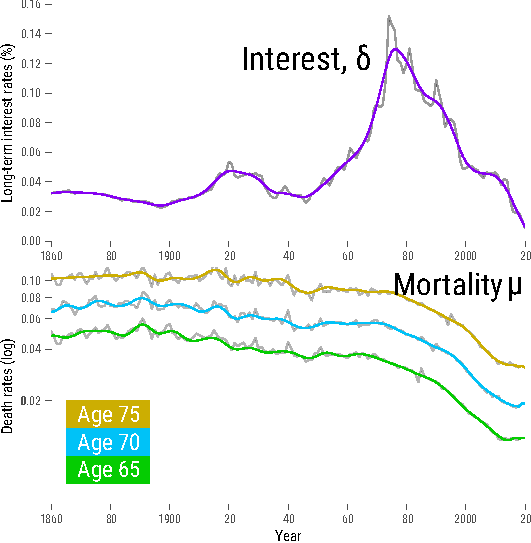
\includegraphics[width=0.7\textwidth]{Fig/Fig1}
	\caption{\textit{Trends over time in interest and mortality rates calculated at ages 65, 70 and 75. Males, 1841-2018.}}
	\label{fig:Fig1}
\end{figure}


How has the value of life annuities changed over time? Figure \ref{fig:Fig2} (upper panel) depict values for $\bar{a}_x(t)$ from 1841 to 2018 for males at age 65. We observe that during the second half of the 19th century and up to the decade of 1940s, $\bar{a}_{65}(t)$ remained at similar levels with small fluctuations. Thereafter, $\bar{a}_{65}(t)$ exhibited a sharp decline up to the decade of 1980s followed by an increasing pattern that has remained until recent years. The lower panel of Figure \ref{fig:Fi2} show the relative derivative of $\bar{a}_{65}(t)$ with respect to time ($\acute{\bar{a}}_{65}(t)$). It is clear that $\acute{\bar{a}}_{65}(t)$ captures well the changes over time in life annuity; positive values indicate that $\bar{a}_{65}(t)$ goes up and negative values indicate a decrease in $\bar{a}_{65}(t)$. In the following sections we analyse the sources of change in the time trend of $\acute{\bar{a}}_{65}(t)$ by making use of the decomposition method developed in Section \ref{sec:timderiv}.

  \begin{figure}[!ht]
  	\centering
  	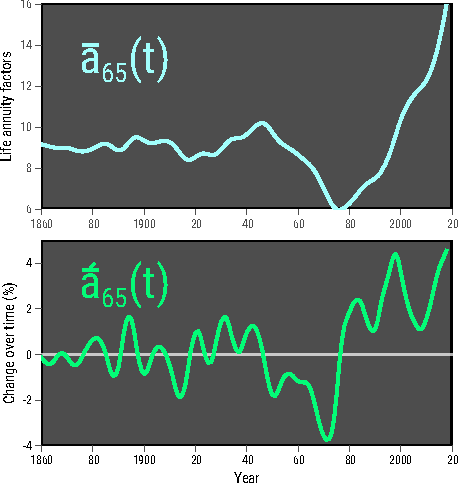
\includegraphics[width=0.7\textwidth]{Fig/Fig2}
  	\caption{\textit{Trends over time in life annuity factors and relative change in $\bar{a}_x(t)$ calculated at age 65. Males, 1841-2018.}}
  	\label{fig:Fig2}
  \end{figure}
  
  

\subsection{Contribution of financial and longevity risks to changes in $\bar{a}_x(t)$}

According to the decomposition formula developed (Equation \ref{eq:TimeDerivC2}), changes over time in $\bar{a}_x(t)$ can be explained in terms of longevity and financial components. Each component depends on the stochastic fluctuations of $\mu(x,t)$ and $\delta(s,t)$ (captured by $\bar{\rho}(t)$ and $\dot{\delta}(t)$ respectively) which are modulated by the sensitivity of $\bar{a}_x(t)$ to changes in the forces of mortality and interest (entropy, ${H}^{p}_x(t)$ and modified duration, ${D}^{c}_x(t)$). Figure \ref{fig:Fig3} depicts all the components responsible of fluctuations over time in $\bar{a}_x(t)$.




\begin{figure}[!ht]
	\centering
	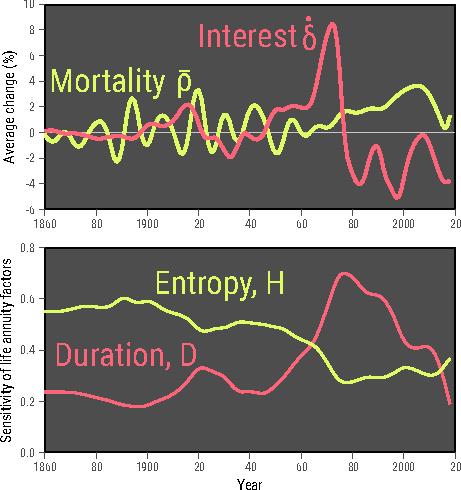
\includegraphics[width=0.7\textwidth]{Fig/Fig3}
	\caption{\textit{Upper panel shows the average change in mortality ($\bar{\rho}(t)$) and interest rates ($\dot{\delta}(t)$). Lower panel shows Entropy ($H$) and modified duration ($D$). Males at age 65, 1841-2018.}}
	\label{fig:Fig3}
\end{figure}


From 1841 to 1940, there were no mortality improvements after age 65 since $\bar{\rho}(t)$ fluctuated around 0\% (upper panel of Figure 3). However, as of 1980s, $\bar{\rho}(t)$ increased steadily indicating an average mortality improvement above age 65 of 2\% and 3\% for the decade of 2000s. In recent years, $\bar{\rho}(t)$ trended downwards, which coincides with the mortality deterioration currently prevailing in the United Kingdom (REF). Regarding changes over time in the force of interest, we observe that $\dot{\delta}(t)$ has also remained at similar levels for most of the observation period with some fluctuations between 1930 and 1950. Since the 1960s, $\dot{\delta}(t)$ went up rapidly reaching the highest increase (of around 8\% in the decade of 1970s). Thereafter, $\dot{\delta}(t)$ declined faster and moved towards negative values entailing a decline in interest rates, which is still ongoing until recent time. Trends in $\bar{\rho}(t)$ and $\dot{\delta}(t)$ are responsible for the time trend we observe in $\bar{a}_x(t)$, which is modulated by the entropy, ${H}^{p}_x(t)$, and modifed duration, ${D}^{c}_x(t)$.


The lower panel of Figure \ref{fig:Fig3} shows that during most of the observation period, ${H}^{p}_x(t)$ was higher than ${D}^{c}_x(t)$. This indicates that $\bar{a}_x(t)$ has been more sensitive to changes in mortality than to changes in interest rates. However, this has changed over time. The entropy show a decreasing trend up to the 1980s where it started to rise. Modified duration, on the other hand, remained somewhat constant over time but as of the 1950s, it trended upwards reaching its maximum in the 1980s (of about 0.8). Thereafter, it decline again. It is worth noting that there are some specific years where ${H}^{p}_x(t)$ and ${D}^{c}_x(t)$ depict the same values. This means that during these years, $\bar{a}_x(t)$ was equally sensitive to changes in mortality and interest rates.


\begin{figure}[!ht]
	\centering
	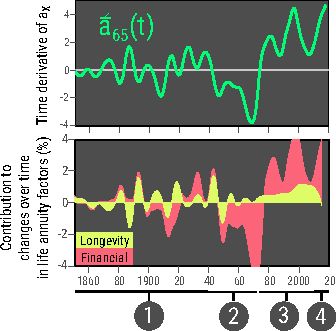
\includegraphics[width=0.6\textwidth]{Fig/Fig4}
	\caption{\textit{Decomposition of changes over time in life annuity factors calculated at ages 65. Males, 1841-2018.}}
	\label{fig:Fig4}
\end{figure}

Using all the measures shown in Figure \ref{fig:Fig3}, we next calculate the contributions of financial ($\dot{\delta}(t){D}^{c}_x(t)$) and longevity risks ($\bar{\rho}(t){H}^{p}_x(t)$) to changes over time in $\bar{a}_{65}(t)$ using the decomposition method developed in Equation \ref{eq:TimeDerivP3}. The upper panel of Figure \ref{fig:Fig4} shows $\acute{\bar{a}}_{65}$\footnote{This is the same as Figure \ref{fig:Fig2}. We show it here so the reader can make sense of the decomposition method} and the lower panel shows the outcome of the decomposition method. Positive/negative values contribute to increase/decrease in $\bar{a}_x(t)$. From Figure \ref{fig:Fig4} it is clear that both, longevity and financial risks have played an important role in the long-term development of $\bar{a}_x(t)$. 

We can distinguish among 4 periods where life annuity factors fluctuated in response to specific changes in financial and longevity risks. From 1841 to 1945, we observe stable annuity factors with contributions of longevity and financial risks to the time trend. In a second period, from 1945 to 1970, we observe decreasing annuity factors mainly driven by the financial component. Around 1970, interest rates reached the highest point, which translates into a negative contribution of the financial component. In the next period, from 1970 to 2015, the time trend changed. Annuity prices went up due to positive contributions of the financial and longevity components. Both, interest and mortality rates went down. In the last period, from 2015 onwards, $\bar{a}_x(t)$ continue to increase with the longevity component contributing less to the trend. This reflects the deceleration of mortality improvements occurring in the UK (REFERENCE).
 
 
 \subsection{Analysis for both sexes and at older ages}
 
 Hitherto, we focused our analysis in trends over time in $\bar{a}_x(t)$ for males calculated at age 65. In Section \ref{sec:olderages} in the Appendix, we extend the analysis to females and to ages 70 and 75 (see Figures \ref{fig:FigA1}, \ref{fig:FigA2}, \ref{fig:FigA3} and \ref{fig:FigA4}). [SHOULD WE INCLUDE THIS SECTION IN THE APPENDIX INSTEAD]
 
  In Figure \ref{fig:FigA1} Sex-specific trends appear to be very similar between sexes with the absolute level of $\bar{a}_x(t)$ for females being slightly higher than the one depicted for males. Similar trends over time also replicate at any onset age of calculation analysed here (e.g. age 65, 70 and 75). However, a closer look reveal that $\bar{a}_x(t)$ changes more abruptly at younger ages (age 65) than at older ages (age 75). This pattern is clear when analysing the time derivative of $\bar{a}_x(t)$ portrayed by $\acute{\bar{a}}_x(t)$  (see Panels C and D of Figure \ref{fig:FigA1}).
  
  
  We observe two regularities from Figure \ref{fig:FigA3}. First, ${H}^{p}_x(t)$ is lower for females than for males whereas ${D}^{c}_x(t)$ is higher for females than for males. This means that, in general, $\bar{a}_x(t)$ for females is less sensitive to $\mu$ and more sensitive to $\delta$ than for males. Second, $\bar{a}_x(t)$ becomes more sensitive to $\mu$ (higher ${H}^{p}_x(t)$) and less sensitive to $\delta$ (lower ${D}^{c}_x(t)$) when calculating $\bar{a}_x(t)$ at older ages. This finding is key to understand how the contributions of longevity and financial risks are moderated differently across ages.
 
 
We observe that longevity contributions to changes in $\bar{a}_x(t)$ are more pronounced in males than in females throughout the whole period of observation. From Figure \ref{fig:FigA4} we observe that the longevity component takes more relevance at older ages. For example, in recent years the longevity component is responsible for a greater contribution of changes in $\bar{a}_{75}(t)$ than for changes in $\bar{a}_{65}(t)$. This pattern is magnified for males. All in all, the analysis performed here provides evidence of the contribution of financial and longevity components to changes in the long-term development of life annuity factors.











\FloatBarrier
\section{Attribution of changes in annuity values across age-groups and terms}

In this section we illustrate how Equation \ref{eq:TimeDerivAge2} can be used to decompose the the one year change in annuity values across the contributions of mortality improvements for different age groups and the change in the term structure of the interest rates. This is in the spirit of the perfomance attribution exercises common in fixed income (see, e.g., \citep{Daul2012}). 

\begin{itemize}
\item Take mortality rates and the term structure for two years (e.g. 1999 and 2000)     
\item  Calculate annuity values for the two years
\item  Calculate the entropy and duration for the different age groups
\item  Plot the profile of duration and entropies (see Exhibit 6-13) of \citep{Ho1992}

\end{itemize}

From Equation \ref{eq:TimeDerivAge2} we can approximate the change in the one year annuity value as 

\begin{equation}\label{eq:ChangeApprox2}
\begin{split}
 \frac{\bar{a}_x(t+1) - \bar{a}_x(t)}{\bar{a}_x(t)} \approx \sum_{i=1}^n\tilde{\rho}_x(t;x_{i-1}, x_i){H}^{p}_x(t;x_{i-1}, x_i) +\sum_{j=1}^m\tilde{\upvarphi}(t;t_{j-1},t_{j}){D}^{p}_x(t;t_{j-1},t_{j}),  
\end{split}
\end{equation} 
 where $\tilde{\rho}_x(t;x_{i-1}, x_i)$ and $\tilde{\upvarphi}(t;t_{j-1},t_{j})$ are the realised mortality improvements and force of interest changes between $t$ and $t+1$.

We can then do a table like Table 3.1 in \citep{Daul2012}


\FloatBarrier
\section{Projection of the decomposition of changes in annuities}









\newpage

\bibliographystyle{apalike}
%\bibliography{/Users/Jesus/Documents/Papers/BibTex/Proposal}
%\bibliography{C:/Users/jmartinez/OneDrive - Syddansk Universitet/Papers/BibTeX/Proposal.bib}

\bibliography{library}

\newpage

\appendix
\section{Appendix}



\subsection{Entropy with constant changes in $\mu(x+s,t)$}\label{sec:EntropyConst}

To measure constant changes we make $\mu(s,t)+\gamma$, then

\begin{equation}\label{eq:EntropyConst1}
\begin{split}
\bar{a}_{x}(t) &= \int_0^\infty{v}(s,t) e^{-\int_{0}^{s} [\mu(x+y,t)+\gamma]dy}ds \\
&= \int_0^\infty {v}(s,t)e^{-\int_{0}^{s} \mu(x+y,t)dy} e^{-\gamma s}ds \\
&= \int_0^\infty {v}(s,t){}_sp_x(t) e^{-\gamma s}ds \\
\end{split}
\end{equation}

We expand $e^{-\gamma s}$ to $1-\gamma s+\frac{\gamma^2}{2} s^{2} +...$, so that


\begin{equation}\label{eq:EntropyConst2}
\begin{split}
\bar{a}_{x}(t) &= \int_0^\infty {}_sp_x(t) {v}(s,t)[1-\gamma s+\frac{\gamma^2}{2} s^{2} +...]ds
\end{split}
\end{equation}

We take the derivative $\bar{a}_{x}(t)$ with respect to $\gamma$ and evaluate $\gamma=0$


\begin{equation}\label{eq:EntropyConst3}
\begin{split}
{H}^{c}_x(t)&=\frac{1}{\bar{a}_x(t)}\frac{\partial \bar{a}_x(t)}{\partial \gamma} \bigg\rvert_{\gamma=0}\\
&= -\frac{\int_0^\infty s {}_sp_x(t) {v}(s,t)ds}{\bar{a}_x(t)} \\
&= \frac{{h}^{c}_x(t)}{\bar{a}_x(t)},
\end{split}
\end{equation}

where ${h}^{c}_x(t)=-\int_0^\infty s {}_sp_x(t) {v}(s,t)ds$



\subsection{Alternative expression for ${H}^{p}_{x}(t)$}\label{sec:EntropyAlt}

\begin{equation} \label{eq:EntropyAnnuityA1}
\begin{split}
{H}^{p}_{x}(t) &= -\frac{ \int_{0}^{\infty}{}_sp_x(t)\ln[{}_sp_x(t)] e^{-\int_{0}^{s}\delta(y,t)dy} ds}{\int_0^\infty {}_sp_x(t) e^{-\int_{0}^{s}\delta(y,t)dy} ds}\\
&= \frac{\int_0^\infty {}_sp_x(t) {v}(s,t) \int_0^s \mu(x+y,t) dy\,ds}{\bar{a}_x(t)}\\
&= \frac{\int_0^\infty  \mu(x+s,t) \int_s^\infty {}_yp_x(t) {v}(y,t)  dy\,ds}{\bar{a}_x(t)}\\
&= \frac{\int_0^\infty  \mu(x+s,t)  {}_sp_x(t) {v}(s,t) \int_s^\infty \frac{ {}_yp_x(t) {v}(y,t)}{ {}_sp_x(t) {v}(s,t)}  dy\,ds}{\bar{a}_x(t)}\\
&=  \frac{\int_0^\infty \mu(x+s,t)   {}_sp_x(t) {v}(s,t) \bar{a}_{x+s}(t) ds}{\bar{a}_x(t)} \\
&=  \frac{\int_0^\infty \mu(x+s,t)  {}_s|\bar{a}_x(t) ds}{\bar{a}_x(t)} \\
&=  \frac{{h}^{p}_{x}(t)}{\bar{a}_x(t)}, \\
\end{split}
\end{equation}

where ${h}^{p}_{x}(t)=\int_0^\infty \mu(x+s,t)   {}_s|\bar{a}_x(t) ds$.



\subsection{Duration with constant changes in $\delta(s,t)$}\label{sec:DurConst}

To measure constant changes we make $\delta(s,t)+\gamma$, then

\begin{equation}\label{eq:DurationConst1}
\begin{split}
\bar{a}_{x}(t) &= \int_0^\infty {}_sp_x(t) e^{- \int_{0}^{s} [\delta(y,t)+\gamma]dy}ds \\
&= \int_0^\infty {}_sp_x(t) e^{- \int_{0}^{s}\delta(y,t)dy}e^{-\gamma s}ds \\
&= \int_0^\infty {}_sp_x(t) {v}(s,t)e^{-\gamma s}ds
\end{split}
\end{equation}

We expand $e^{-\gamma s}$ to $1-\gamma s+\frac{\gamma^2}{2} s^{2} +...$, so that


\begin{equation}\label{eq:DurationConst1}
\begin{split}
\bar{a}_{x}(t) &= \int_0^\infty {}_sp_x(t) {v}(s,t)[1-\gamma s+\frac{\gamma^2}{2} s^{2} +...]ds
\end{split}
\end{equation}

We take the derivative $\bar{a}_{x}(t)$ with respect to $\gamma$ and evaluate $\gamma=0$


\begin{equation}\label{eq:DurationConst2}
\begin{split}
{D}^{c}_x(t)&=-\frac{1}{\bar{a}_x(t)}\frac{\partial \bar{a}_x(t)}{\partial \gamma} \bigg\rvert_{\gamma=0}\\
              &= \frac{\int_0^\infty s {}_sp_x(t) {v}(s,t)ds}{\bar{a}_x(t)} \\
              &= \frac{{d}^{c}_x(t)}{\bar{a}_x(t)},
\end{split}
\end{equation}

where ${d}^{c}_x(t)=\int_0^\infty s {}_sp_x(t) {v}(s,t)ds$



\subsection{Duration with proportional changes in $\delta(s,t)$} \label{sec:DurProp}

To calculate duration with proportional changes in $\delta(s,t)$, we assume that $\gamma$ is a small number such that $\delta(s,t)(1+\gamma)$ and  ${v}(s,t)=e^{-\int_0^{s}  \delta(y,t)(1+\gamma)dy}$.


\begin{equation}\label{eq:DurationProp1}
\begin{split}
\bar{a} _x(t) &= \int_0^\infty {}_sp_x(t) e^{-\int_0^{s}\delta(y,t)(1+\gamma)dy}ds \\
&= \int_0^\infty {}_sp_x(t) e^{-\int_0^{s}\delta(y,t)dy}e^{-\int_0^{s}\delta(y,t)\gamma dy}ds \\
&= \int_0^\infty {}_sp_x(t) v(s,t)v(s,t)^{\gamma}ds \\
\end{split}
\end{equation}


We expand $v(s,t)^{\gamma}$ to $1+\ln(v(s,t)) \gamma+{\ln(v(s,t))}^2 \frac{\gamma^2}{2}+...$, so that


\begin{equation}\label{eq:DurationProp2}
\begin{split}
\bar{a}_x(t) &= \int_0^\infty {}_sp_x(t) s(y,t)[1+\ln(v(s,t)) \gamma+{\ln(v(s,t))}^2 \frac{\gamma^2}{2}+...]ds\\
\end{split}
\end{equation}


To calculate the duration ${D}^{p}_{x}(t)$ we take the derivate of the expression above with respect to $\gamma$ and make $\gamma=0$

\begin{equation}\label{eq:DurationProp3}
\begin{split}
{D}^{p}_{x}(t)&=-\frac{1}{\bar{a}_x(t)}\frac{\partial \bar{a}_x(t)}{\partial \gamma} \bigg\rvert_{\gamma=0} \\
&= -\frac{\int_0^\infty {}_sp_x(t) v(s,t) \ln(v(s,t))ds}{\bar{a}_x(t)} \\
\end{split}
\end{equation}


Equation \ref{eq:DurationProp3} can be re-expressed as 


\begin{equation}\label{eq:DurationProp4}
\begin{split}
{D}^{p}_{x}(t) &= -\frac{\int_0^\infty {}_sp_x(t) v(s,t) \ln(v(s,t))ds}{\bar{a}_x(t)}\\
&= \frac{\int_0^\infty {}_sp_x(t) v(s,t) \int_0^{s} \delta(y,t)dy ds }{\bar{a}_x(t)}\\
&= \frac{\int_0^\infty \delta(s,t)  \int_{s}^{\infty} {}_{y}p_x(t) v(y,t)dy ds }{\bar{a}_x(t)}\\
&= \frac{\int_0^\infty \delta(s,t) {}_sp_x(t) v(s,t) \bar{a}_{x+s}(t)  ds }{\bar{a}_x(t)}\\
&= \frac{\int_0^\infty \delta(s,t) {}_s|\bar{a}_x(t) ds}{\bar{a}_x(t)} \\
&= \frac{{d}^{p}_{x}(t)}{\bar{a}_x(t)}.
\end{split}
\end{equation}



where ${d}^{p}_{x}(t)=\int_0^\infty \delta(s,t) {}_s|\bar{a}_x(t) ds$.


\subsection{Historical decomposition of life annuities: both sexes at ages 65, 70 and 75} \label{sec:olderages}


\begin{figure}[!ht]
	\centering
	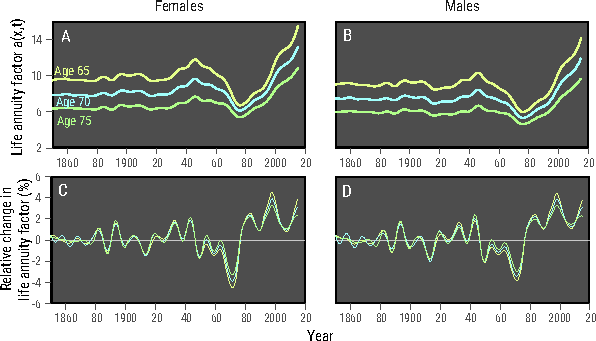
\includegraphics[width=1\textwidth]{Fig/FigA1}
	\caption{\textit{Trends over time in life annuity factors and relative change in $\bar{a}_x(t)$ calculated at ages 65, 70 and 75. Both sexes, 1841-2018.}}
	\label{fig:FigA1}
\end{figure}




\begin{figure}[!ht]
	\centering
	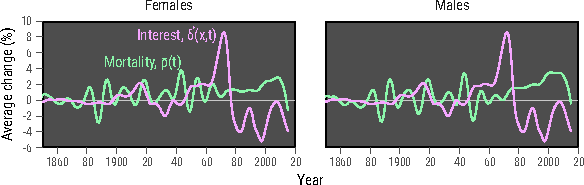
\includegraphics[width=1\textwidth]{Fig/FigA2}
	\caption{\textit{Average change in mortality ($\bar{\rho}(t)$) calculated for all ages above age 65 and rate of change in interest rates ($\dot{\delta}(t)$). Note that $\dot{\delta}(t)$ is expressed in basis points to ease readability. Both sexes, 1841-2018.}}
	\label{fig:FigA2}
\end{figure}




\begin{figure}[!ht]
	\centering
	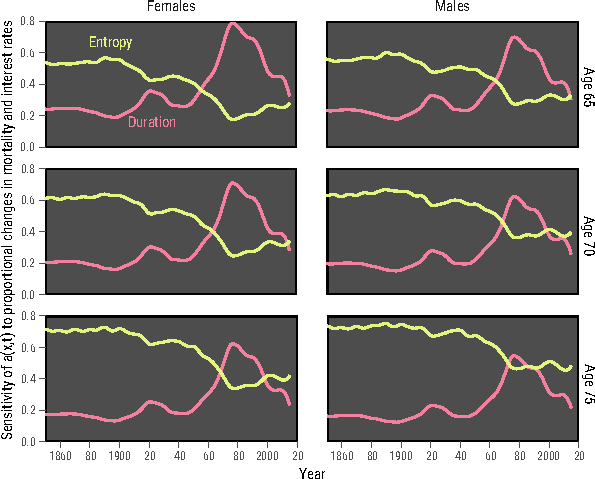
\includegraphics[width=1\textwidth]{Fig/FigA3}
	\caption{\textit{Entropy and modified duration assuming proportional changes calculated at ages 65, 70 and 75. Both sexes, 1841-2018.}}
	\label{fig:FigA3}
\end{figure}






\begin{figure}[!ht]
	\centering
	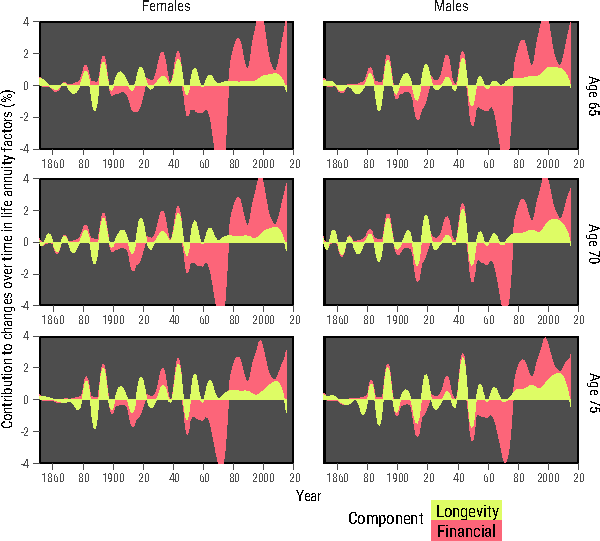
\includegraphics[width=1\textwidth]{Fig/FigA4}
	\caption{\textit{Decomposition of changes over time in life annuity factors calculated at ages 65, 70 and 75. Both sexes, 1841-2018.}}
	\label{fig:FigA4}
\end{figure}











\end{document}
